\chapter{Experimental setup and tests on board}
\section{Introduction}
This chapter will focus on the firmware validation procedures and on the devices used for this purpose. The first half of the chapter will be dedicated to the test bench setup, the ABACUS\_v2 test board and other hardware devices involved. The second half will analyse how the new addition to the firmware perform in real world; this means that trimming DAC configuration test, latch data taking and timestamp measurement have been performed with success.

\section{Experimental setup}\label{testbench}
\begin{figure}[H]
	\centering
	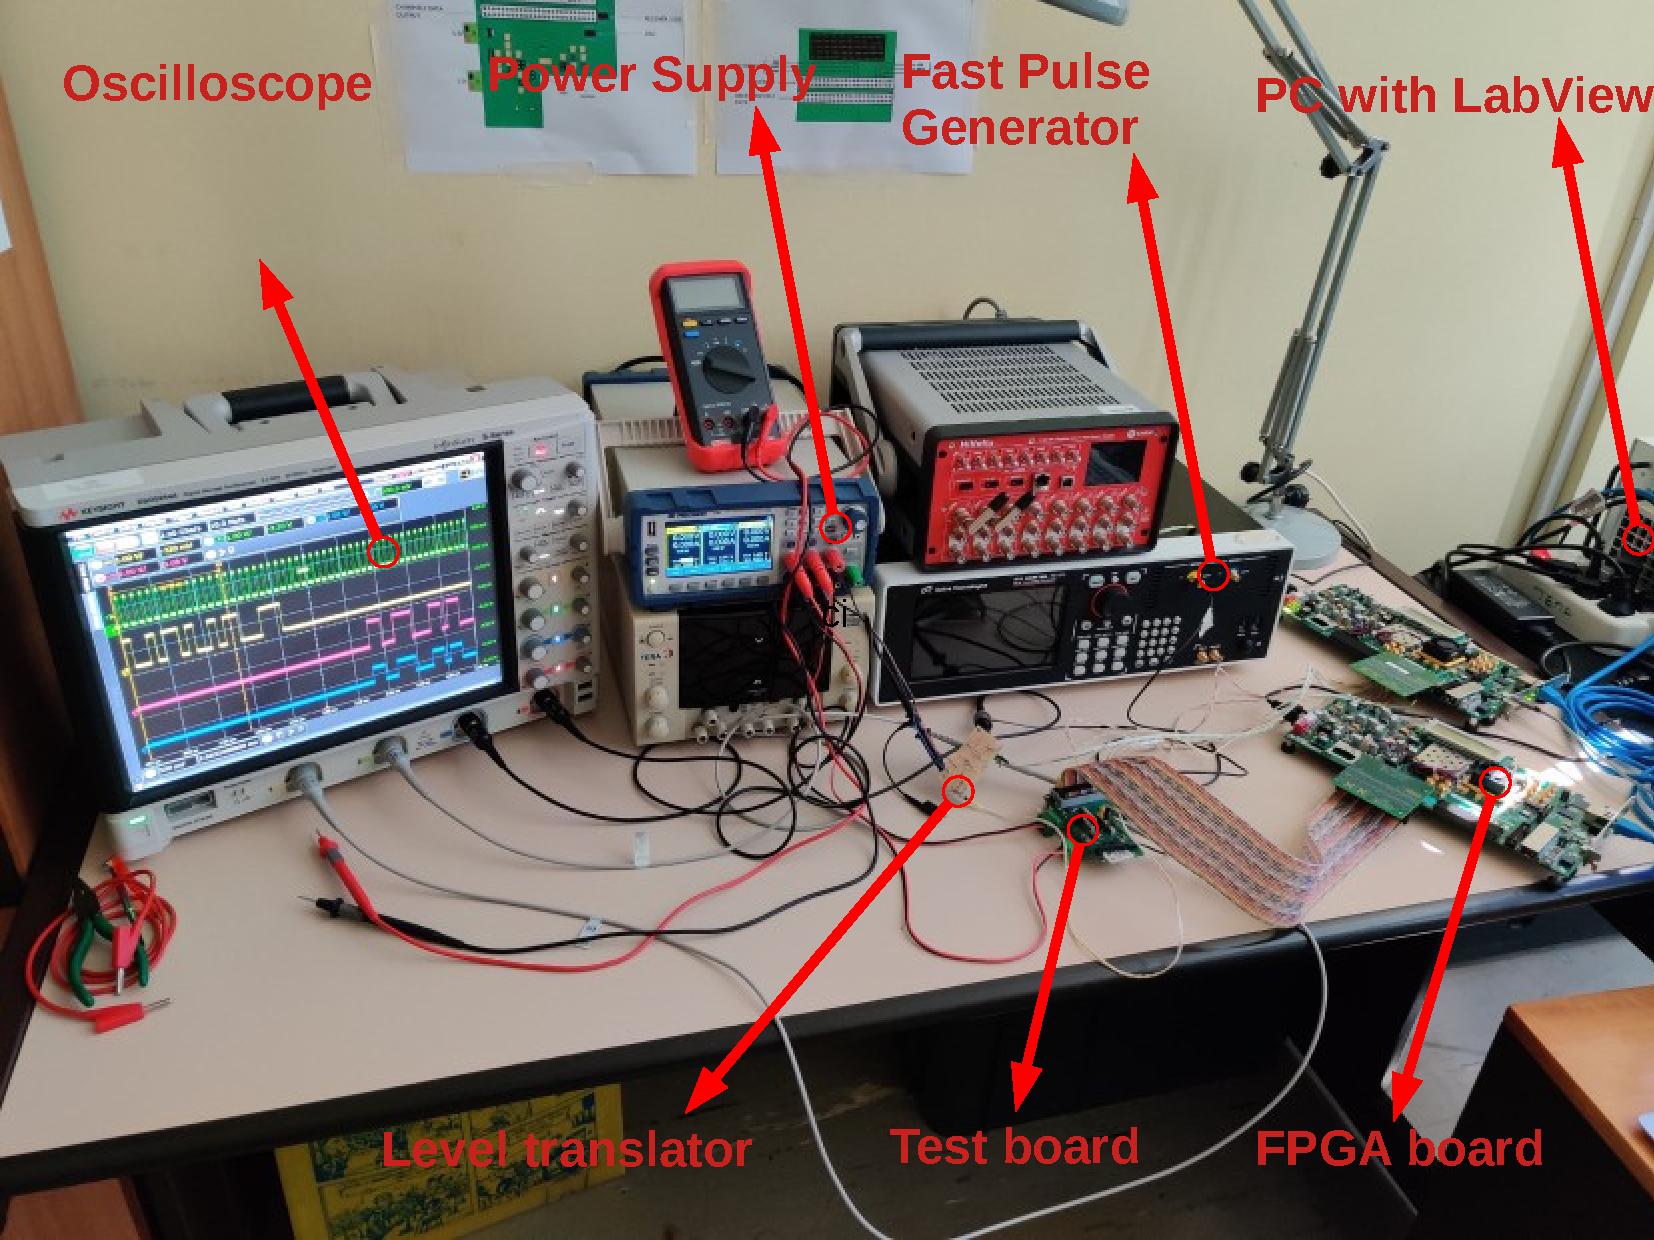
\includegraphics[width=0.7\linewidth]{IMG/ch5/TESTBENCH}
	\caption{Experimental setup and devices}
	\label{fig:testbench}
\end{figure}
In order to properly validate the new additions of the FPGA firmware, after the simulations performed in the Vivado design suite, numerous tests have been carried out on the FPGA board and on chip.
The setup used to perform the test is shown in figure \ref{fig:testbench} and it comprehends:
\begin{itemize}
	\item A \textit{KEYSIGHT DSOS254A} (Digital Storage Oscilloscope), 4-channels, 2.5~GHz, 20~GSa/s, 10~bit ADC professional oscilloscope
	\item A \textit{BK PRECISION 9140} power supply for the test board and the level translator device of section \ref{leveltranslator}
	\item A \textit{ACTIVE TECHNOLOGIES} Fast Pulse Generator (70~ps Pulse/Delay) used to simulate the signal coming from the detector
	\item A computer with LabVIEW 
	\item The FPGA board with the NEW firmware that needs to be tested
	\item The test board with the ABACUS\_v2 bonded to it
	\item A level translator device that will be explained better in the next pages
\end{itemize}
\noindent Those are the main devices involved in FPGA firmware test, however it is obvious that when dealing with complex electronics and prototype chips many more smaller and less important tools are used for debug purpose. Hand-tools, cables, switches and other less important things will be ignored in the future sections.

\section{Test board}\label{testboard}
\begin{figure}[H]
	\centering
	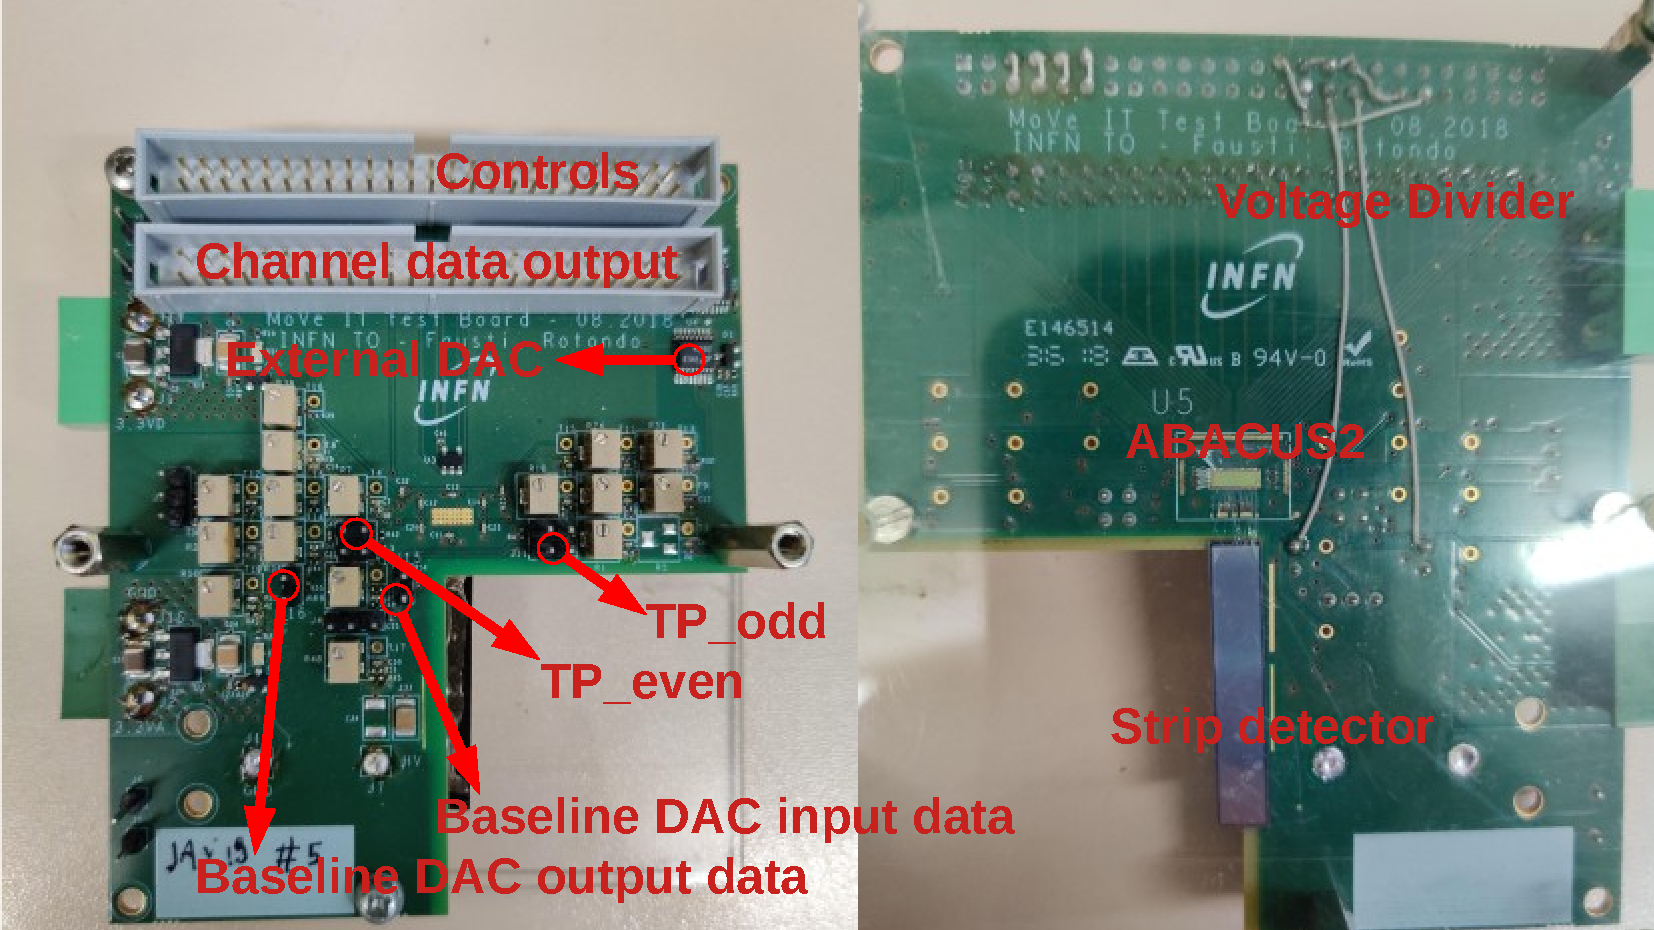
\includegraphics[width=0.9\linewidth]{IMG/ch5/TESTBOARD}
	\caption{Test board top and bottom view}
	\label{fig:testboard}
\end{figure}
To test every feature of the ABACUS\_v2 chip the INFN Turin section projected and created a test board.
On the back side of the PCB, shown in figure \ref{fig:testboard}, it can be observed the naked chip bonded to the board.
Moreover, the main components of the test board are:
\begin{itemize}
	\item Two 50 pin connectors, the bottom one is used to send the bipolar data from the chip to the FPGA and the top one is used to receive the controls (main DAC, trimming DACs, clocks) to the board
	\begin{figure}[H]
		\centering
		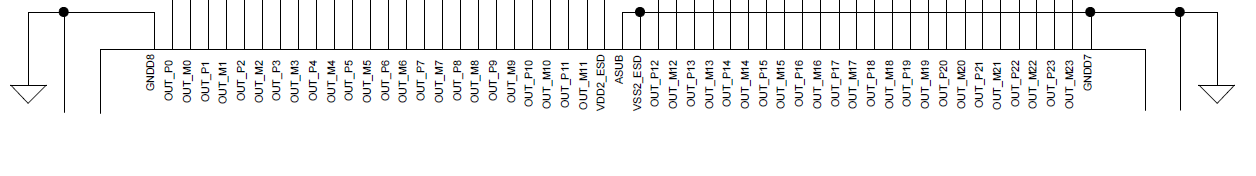
\includegraphics[width=0.95\linewidth]{IMG/ch5/DATATOFPGA}
		\caption{Wiring from the chip to the bottom 50 PIN connector}
		\label{fig:datatofpga}
	\end{figure}
	\item The external DAC, a commercially available Linear Technology LTC2604 \cite{LTC2604} Quad 16-bit Rail-to-Rail DAC, connected as in figure \ref{fig:externaldac}
	\begin{figure}[H]
		\centering
		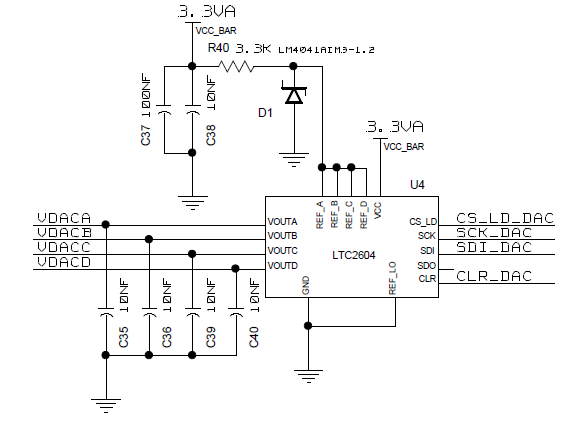
\includegraphics[width=0.3\linewidth]{IMG/ch5/EXTERNALDAC}
		\caption{Connections of the LTC2604 external DAC}
		\label{fig:externaldac}
	\end{figure}
	\item Two TP (Test Pulse) connectors (\textit{TP\_odd} and \textit{TP\_even}) used to inject a charge and thus simulate the signal from the LGAD detector, connected to the chip as in figure \ref{fig:tpconnector}
	\begin{figure}[H]
		\centering
		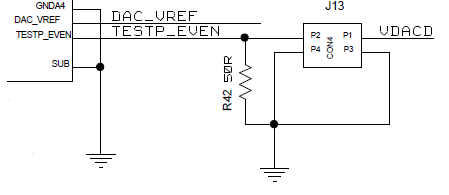
\includegraphics[width=0.4\linewidth]{IMG/ch5/TPCONNECTOR}
		\caption{Wiring of the \textit{TP\_even} connector}
		\label{fig:tpconnector}
	\end{figure}
	\item Two connectors (Baseline DAC input data and Baseline DAC output data) used to send and receive data from the internal DACs, wired as in figure \ref{fig:internaldacwiring} with a 50~$\Omega$ termination 
	\begin{figure}[H]
		\centering
		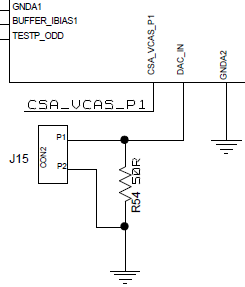
\includegraphics[width=0.2\linewidth]{IMG/ch5/INTERNALDACWIRING}
		\caption{Wiring of the Baseline (trimming/internal) DAC data in connector}
		\label{fig:internaldacwiring}
	\end{figure} 
\end{itemize} 
\noindent The 50 PIN connector is connected to the FMC port by means of a breakout board that can be seen attached to the FPGA in figure \ref{fig:testbench}. This adapter PCB has no electrical components, only wiring to adapt one physical connector to another.
To be noted that the ABACUS\_v2 test board has many trimmers and test pads. These are used to regulate and measure different voltages of the device. This is mandatory for a proper characterization of the ASIC.
\section{Hardware devices}\label{hardware}
\noindent As described previously the ABACUS\_v2 chip, for the configuration and readout of the internal DACs, works on 1,2~V LVCMOS single-ended signal only. however the FPGA uses only one reference voltage for the entire FMC connector at 2.5~V, this means that for how the board is configured it is impossible to send and receive 1,2~V signals.
In order to solve this problem two simple devices have been implemented; a voltage divider and a level translator device.
\subsection{Voltage divider}
The data coming from the FPGA to the chip is at 2,5~V single-ended. To lower this value two simple voltage divider were implemented with 2 SMD (Surface-Mount Devices) and a $\frac{1}{4}$~W ceramic resistor each on the back of the test board; this can be seen in figure \ref{fig:voltagedivider} and \ref{fig:testboard}.
\begin{figure}[H]
	\centering
	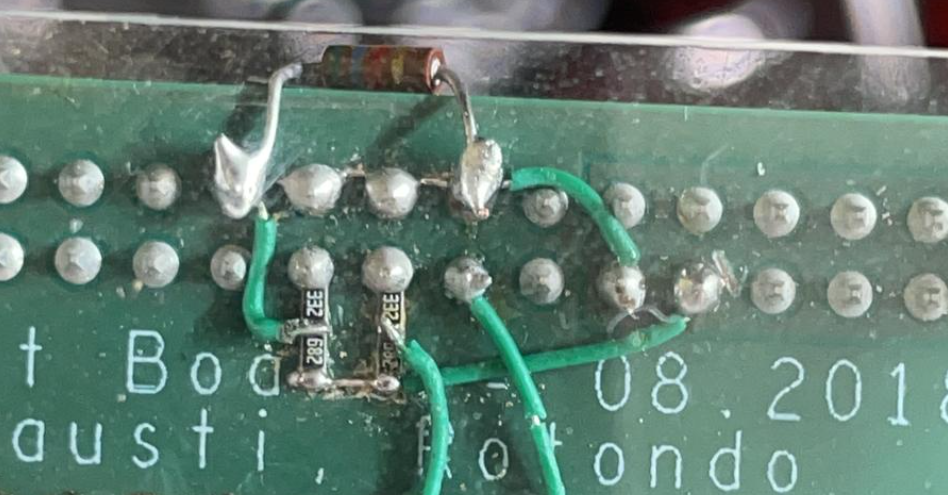
\includegraphics[width=0.6\linewidth]{IMG/ch5/VOLTAGEDIVIDER}
	\caption{Voltage dividers on the back of the test board, one is used for the clock signal and one for the data input}
	\label{fig:voltagedivider}
\end{figure}
\noindent To obtain the 1.2~V output voltage three resistors were used; a 3.3~k$\Omega$ one for the first stage and a 6.8~k$\Omega$ and 5.6~k$\Omega$ placed in parallel for the second stage.
\subsection{Level translator}\label{leveltranslator}
The data coming from the chip is at 1.2~V. This value is too low and thus the board reads it always as \textit{low}. A voltage translation device is mandatory in order to boost the signal \textit{high} value.
\begin{figure}[H]
	\centering
	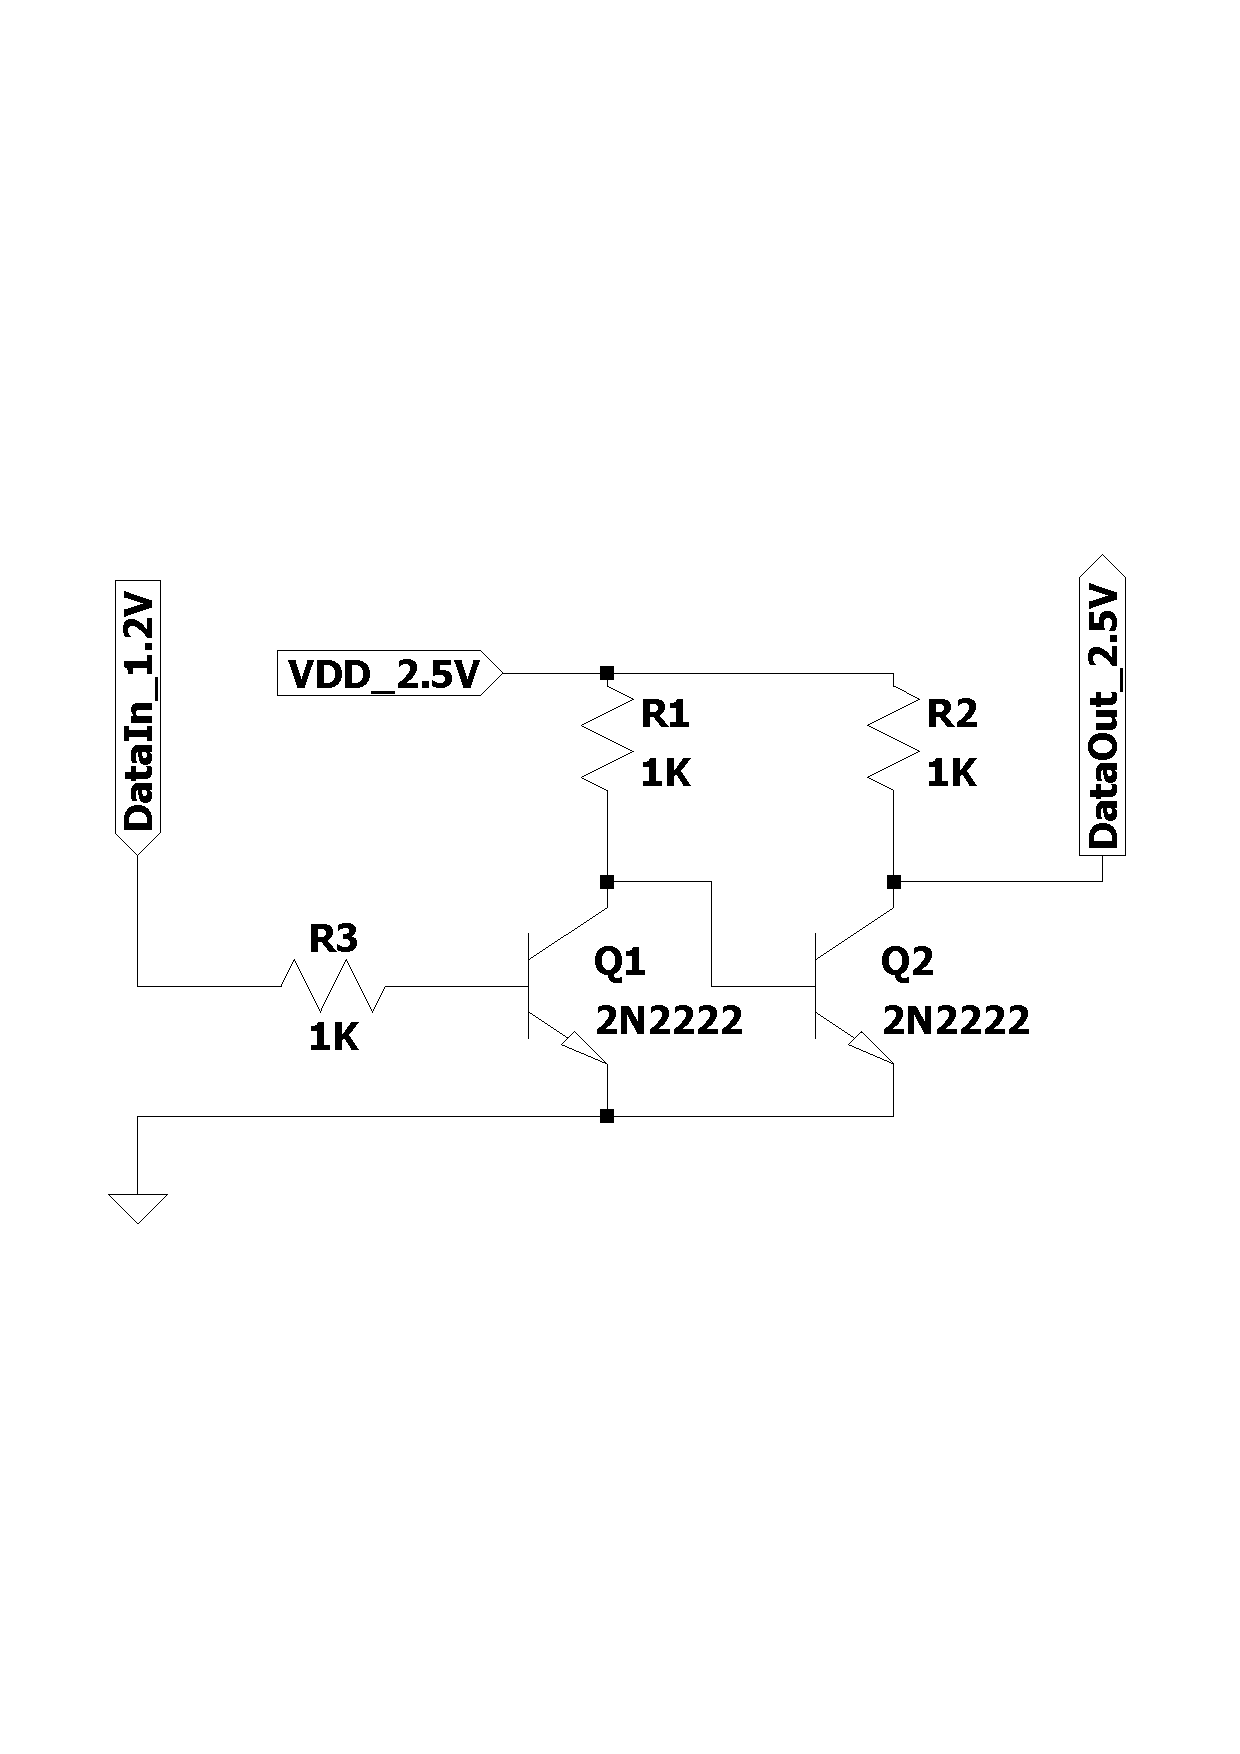
\includegraphics[width=0.6\linewidth]{IMG/ch5/DIAGRAM}
	\caption{Diagram of the level translation device}
	\label{fig:diagram}
\end{figure}
\noindent For this purpose I created the simple circuit that can be seen in figure \ref{fig:diagram} using three 1~k$\Omega$ resistor and two classic \textit{2N2222} transistors that are configured in the standard common emitter mode.
This device has been simulated using LTspice simulator and the results can be seen in figure \ref{fig:transsimulation}.
The green signal is the input data at 1.2~V while the purple one is the output signal at 2.5~V.
According to the simulation the device works properly and thus it can be implemented in hardware.
\begin{figure}[H]
	\centering
	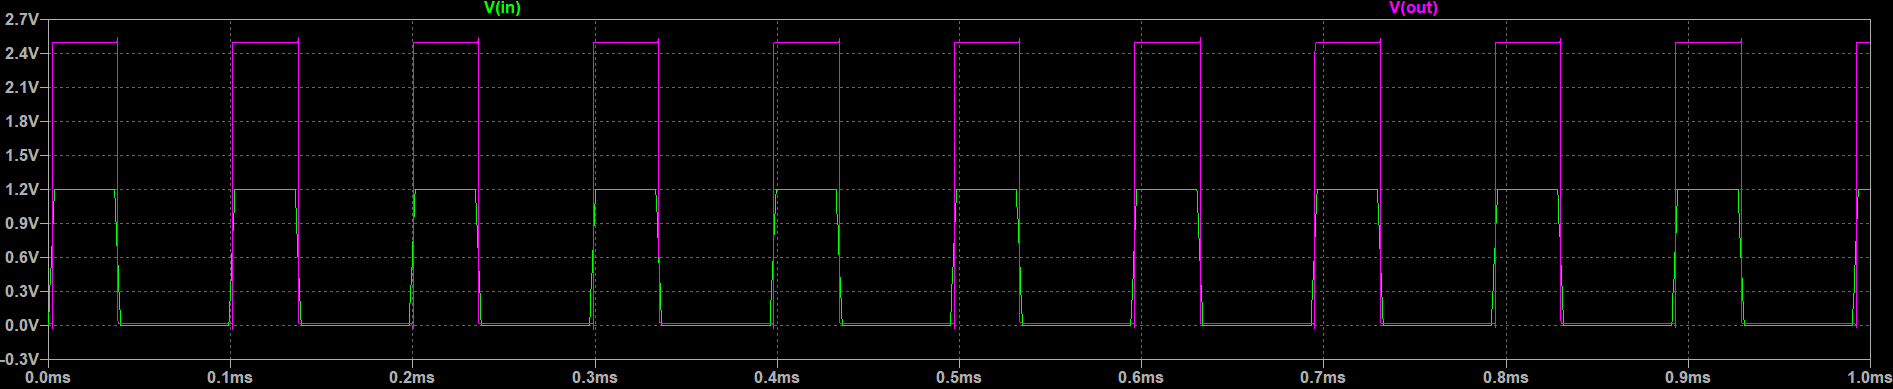
\includegraphics[width=1\linewidth]{IMG/ch5/TRANSSIMULATION}
	\caption{LTspice simulation of the translation device}
	\label{fig:transsimulation}
\end{figure}
\noindent The device was built soldering the components on a piece of perfboard that can be seen in figure \ref{fig:fronttranslator} and \ref{fig:backtranslator}.
It need to be powered externally with 2.45~V and, in order to assure the safety of the FPGA, the current was limited to 0.05~A. 
\begin{figure}[H]
	\centering
	\begin{minipage}{.5\textwidth}
		\centering
		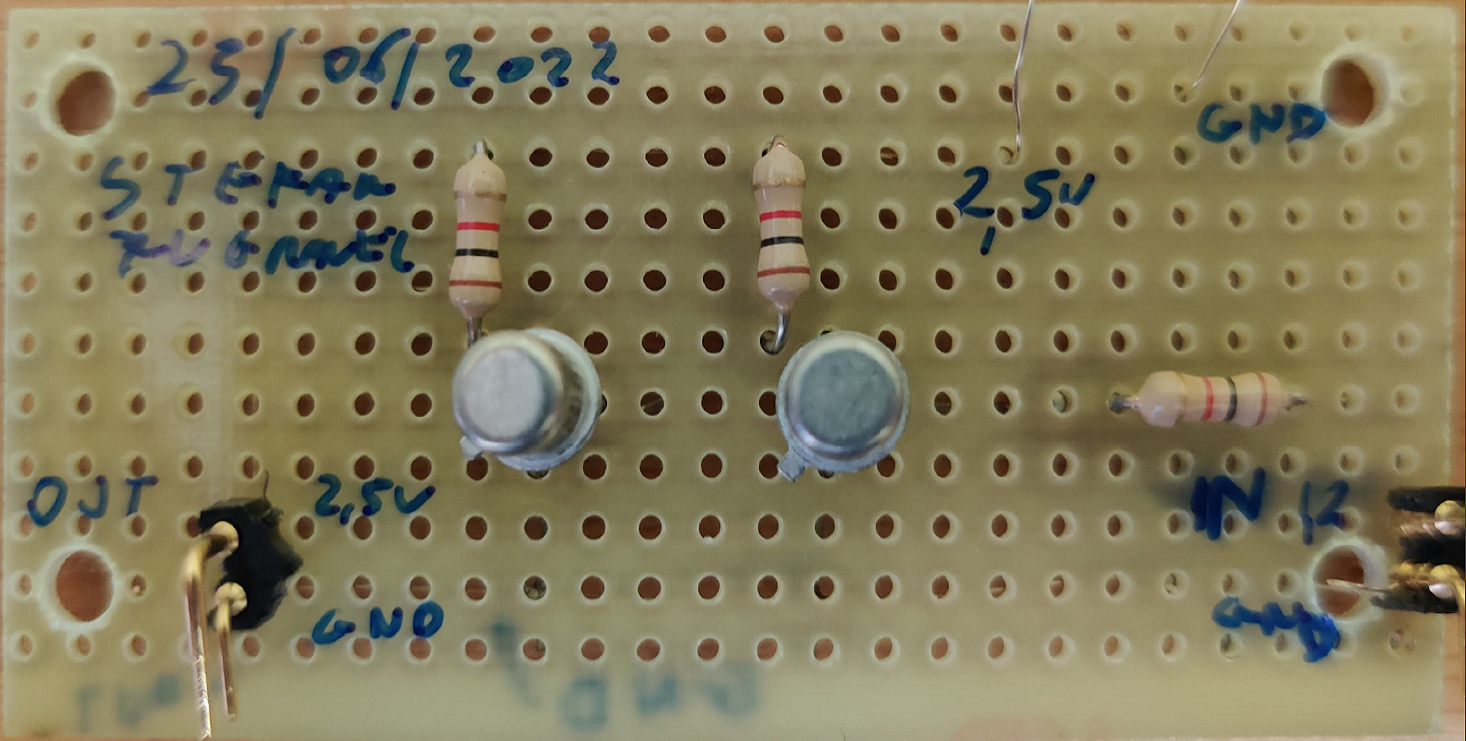
\includegraphics[width=.99\linewidth]{IMG/ch5/FRONTTRANSLATOR}
		\caption{Front view of the \\implemented translation device}
		\label{fig:fronttranslator}
	\end{minipage}%
	\begin{minipage}{.5\textwidth}
		\centering
		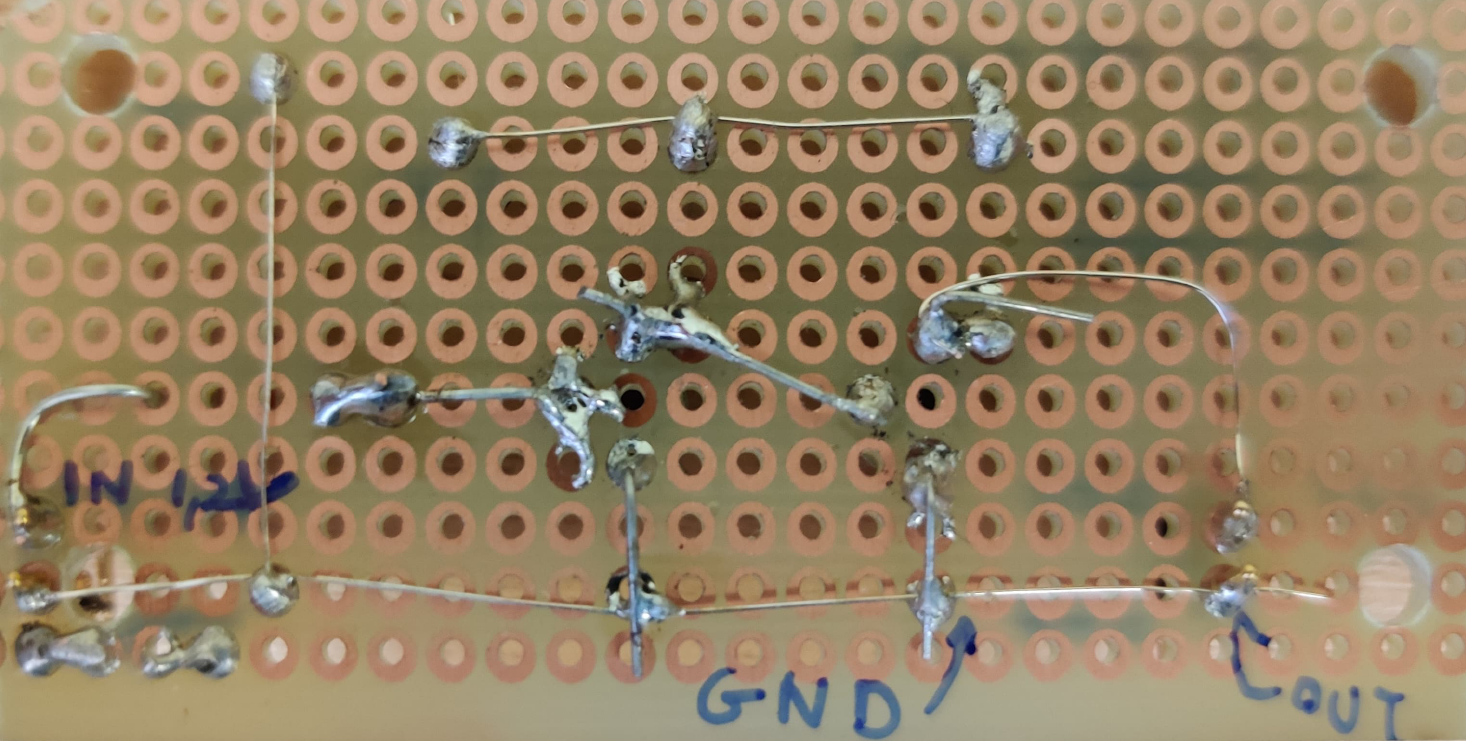
\includegraphics[width=.99\linewidth]{IMG/ch5/BACKTRANSLATOR}
		\caption{Back view of the \\implemented translation device}
		\label{fig:backtranslator}
	\end{minipage}
\end{figure}

\section{Firmware validation on board}
The validation of the firmware was performed in two separate moments, the first one was done in May 2021 and tested the trimming DACs, while the second one was carried out in October 2021 and validated the latch system and the timestamp generator. 
\subsection{Trimming DAC test}\label{dactests}
The trimming DAC validation process was divided into three parts, the verification of the clock period and the amplitude of the signal, the verification of the writing sequence and finally the verification of the reading process. 
All this tests were performed with the FPGA connected to the ABACUS\_v2 test board and the relevant signals were probed with the oscilloscope. The test board was powered with two 3.3~V rails.
\subsubsection{Clock and amplitude}
For this first part the goal was to validate the clock period and its amplitude. In order to do that a write non-specified command was sent while probing the \textit{baseline\_dac\_sck} signal. 
\begin{figure}[H]
	\centering
	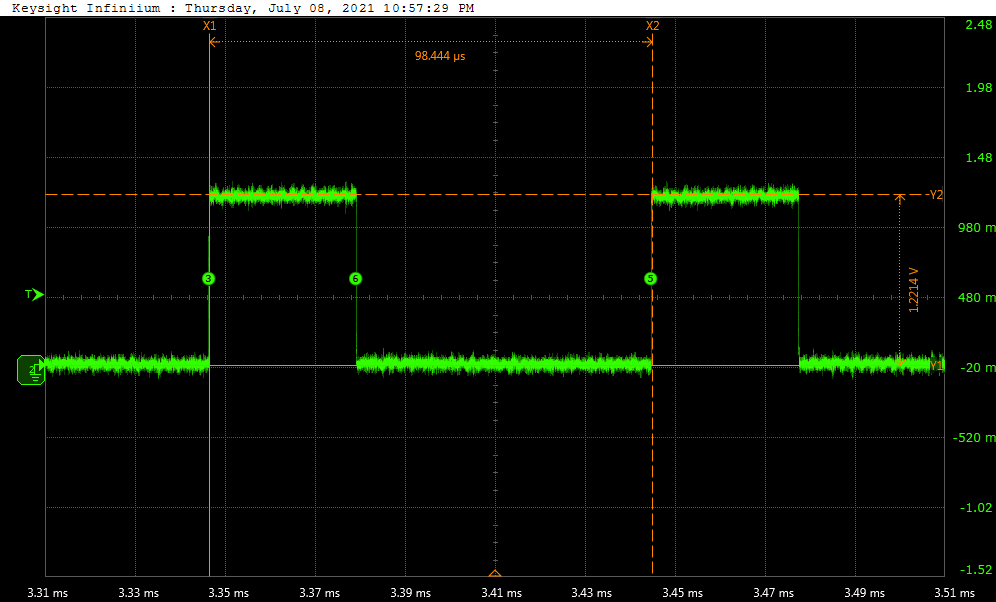
\includegraphics[width=0.7\linewidth]{IMG/ch5/probe/09-08-2021_clock-specks}
	\caption{\textit{baseline\_dac\_sck}; period and amplitude measurements}
	\label{fig:clockspecs}
\end{figure}
\noindent In section \ref{confing} it was said that the clock period should theoretically be 98.28~$\mu$s, in figure \ref{fig:clockspecs} it can be seen that the measured period is 98.44~$\mu$s. The difference between the two values is 160~ns which is approximately $\approx$0.16\% of the total. The period can then be considered perfectly compatible considering that the cursor positioning was done manually and thus the human error must be considered too.
The second value to be noted in figure \ref{fig:clockspecs} is that the amplitude of the signal is 1.22~V, this is perfectly safe for the chip. 

\subsubsection{Write command}
\noindent In order to write into the trimming DACs and read from them a new labview panel was made by \textit{Emanuele Data}\cite{data}. This piece of software can be seen in figure \ref{fig:labview3} sends the commands discussed in section \ref{InternalDac}. In addition it implements some useful features like:
\begin{itemize}
	\item The ability to write on only one DAC at the time with the \textit{Set Internal DAC} button.
	\item The ability to write every DAC with a single \textit{Set multiple internal DAC} button press.
	\item The possibility to read only one DAC value at the time with the \textit{Read ONE Internal DAC} button.
	\item The possibility to read every DAC with a single \textit{Read Internal DACs} button press.
	\item The ability to chose for each DAC channel if the signal needs to be sent to the HPC or LPC FMC.
\end{itemize}
\begin{figure}[H]
	\centering
	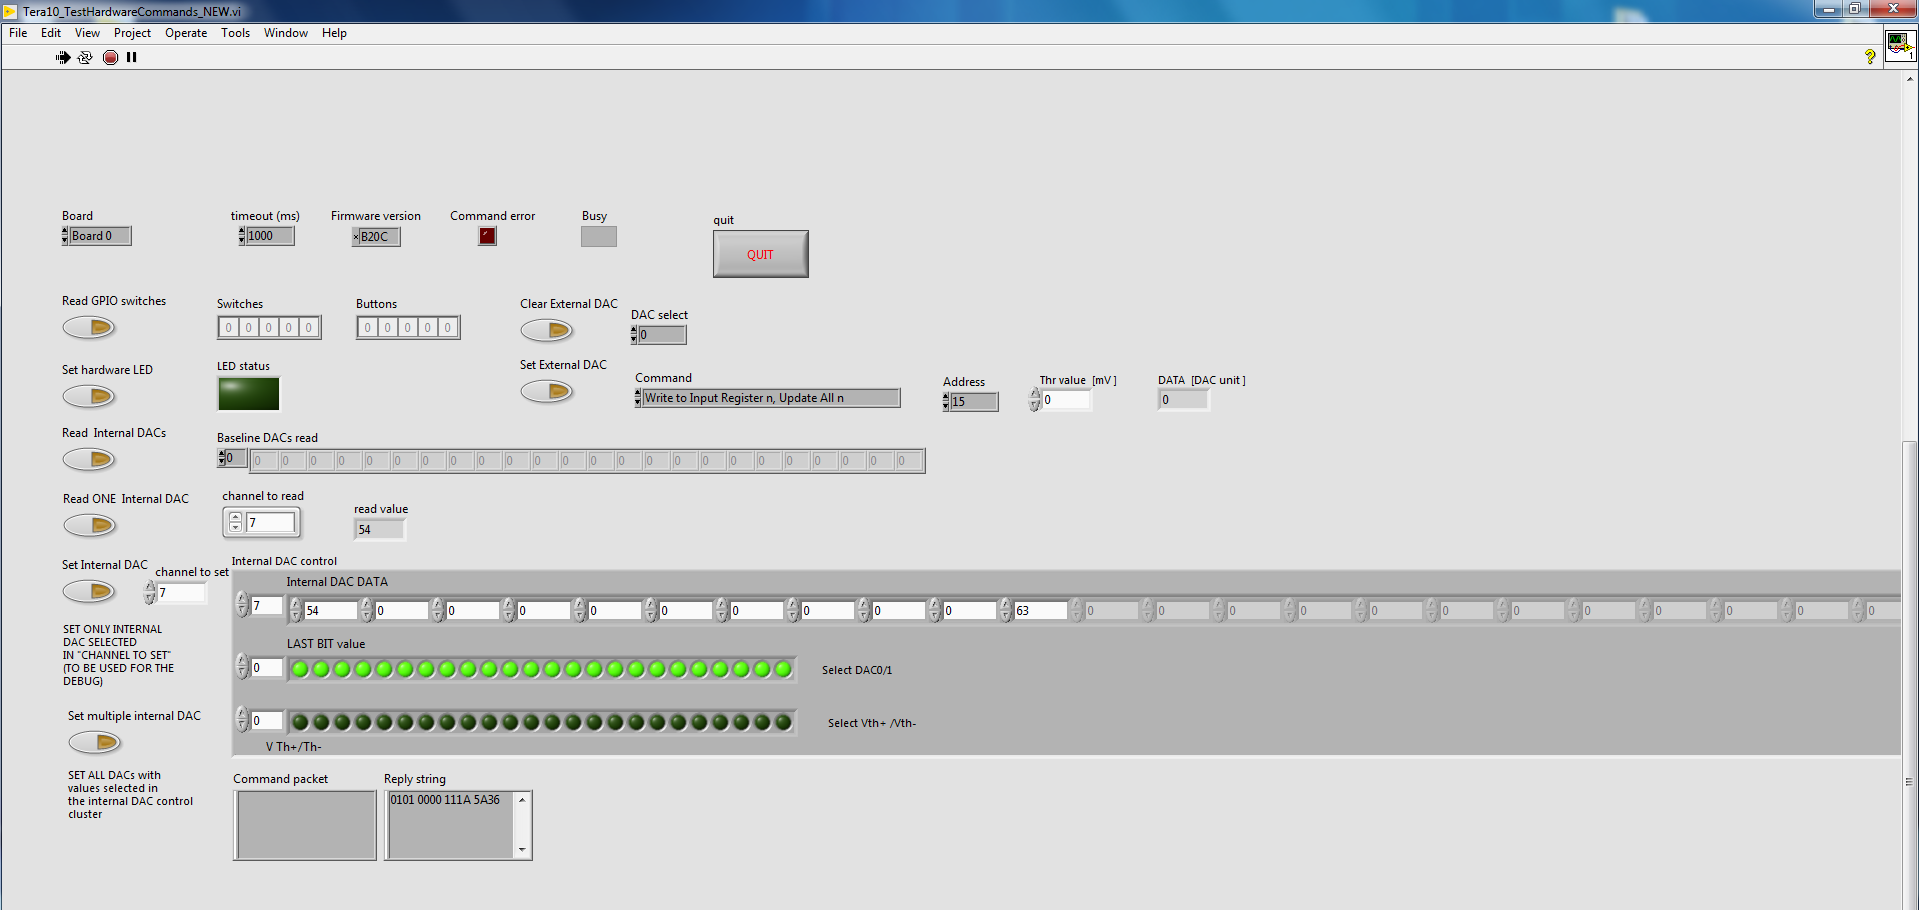
\includegraphics[width=0.99\linewidth]{IMG/ch3/LABVIEW2}
	\caption{LabVIEW tool coded by \textit{Emanuele Data} for the configuration of the trimming DACs}
	\label{fig:labview3}
\end{figure}
\begin{figure}[H]
	\centering
	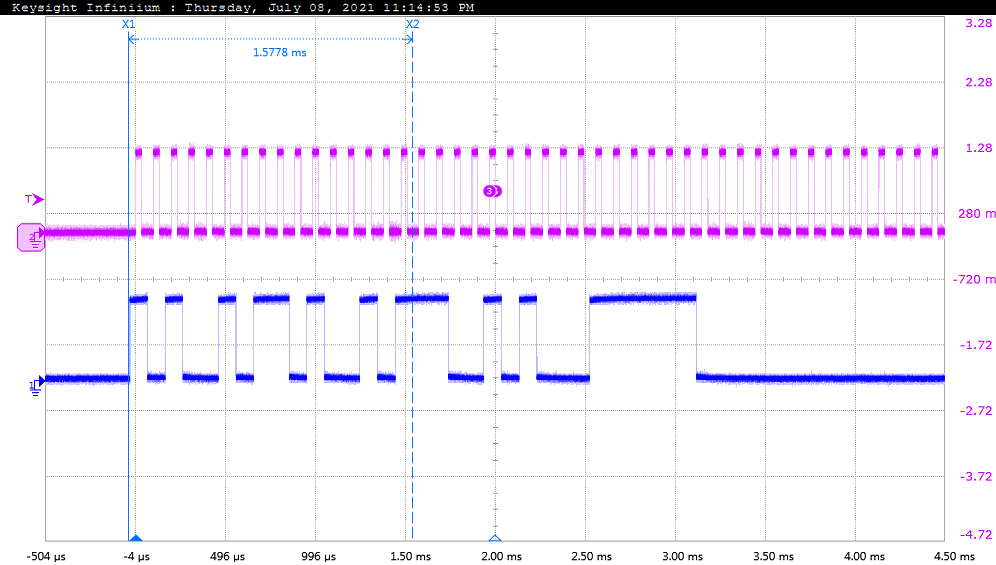
\includegraphics[width=0.7\linewidth]{IMG/ch5/probe/09-08-2021_ch05-write63-baselinedac1}
	\caption{Writing sequence, channel 5, word 63, DAC 1\\{\color{green}green}= clock, {\color{yellow}yellow}= data out}
	\label{fig:ch05write63}
\end{figure}
\noindent In figure \ref{fig:ch05write63} it can be seen a reading sequence being sent to the chip. In green there is the clock signal discussed previously while in yellow it can be seen the serial data being sent to the DAC controller.
Each horizontal square is 0.5~ms, while each vertical square is 1~V (the signals were probed after the voltage divider). 
Between the two markers there is the initialization sequence that needs to be always sent, this is 0xA5A5~=~0b1010-0101-1010-0101.
Immediately after that there are the two command bits, in this case (Writing) their are 0b11.
Next in sequence there is the 6~bit channel address that is divided into a 5~bit address plus a 1~bit V$_{th}$ selector, that for this version of the chip is not used thus is always zero.
The remaining 5~bits are 0d5~=~0b0-0101 thus channel 5. The remaining 8~bits are divided into 2 not used bits (the MSB) and 6 data bits.
In this case these bits are 0d63~=~0b0011-1111, the maximum possible value for a 6~bit DAC.
After this the clock continues for 16 more cycles while the data stays \textit{low}.
For the moment the user has no way of knowing if the chip was properly configured because it does not sends any feedback while writing. In order to verify if the DACs are properly setted a reading procedure needs to be carried out. This will be analysed in the next subsection.  

\subsubsection{Read command}
\begin{figure}[H]
	\centering
	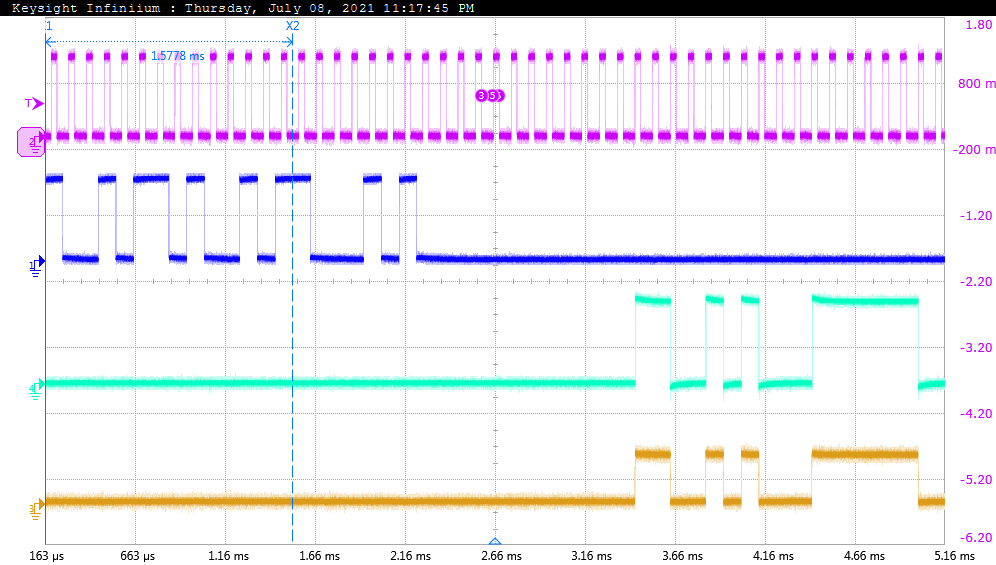
\includegraphics[width=0.7\linewidth]{IMG/ch5/probe/09-08-2021_ch05-read63-baselinedac1}
	\caption{Reading sequence, channel 5, word 63, DAC 1\\{\color{green}green}= clock, {\color{yellow}yellow}= data out,\\{\color{red}red}= data in, {\color{blue}blue}= data from chip}
	\label{fig:ch05read63}
\end{figure}
\noindent In figure \ref{fig:ch05read63} it can be seen a reading sequence being performed on the same channel as before (ch05).
In green there is the clock signal, in yellow it can be seen the serial data being to the chip, in blue there is the data going from from the chip to the level translator and in red there is the data from the level translator to the FPGA.
Each horizontal square is 0.5~ms, while each vertical square is 1~V for the green and yellow signals and 2~V for the red and blue signals.
Between the two markers there is the initialization sequence 0xA5A5~=~0b1010-0101-1010-0101, after that there is the 2-bit read command 0b10 and next there is the address to be read, in this case channel 5, thus 0d5~=~0b0-0101 as before.
When sending a read command the 8~bit data are not considered; this firmware drives them \textit{low}.
The output from the chip is at 1.2~V, too low to be read by the board, for this reason the signal is boosted by the level translator shown in section \ref{leveltranslator} up to 2.5~V (in red).
The data sent by the chip is made up by 16~bit words. The first 2~bit are a \textit{"read confirmation"} signal 0b11. The next 6 bit are the confirmation of the selected channel, it this case 0d5~=~0b0-0101 plus 0b0 for the V$_{th}$ selector.
The chip is reading from the same channel that was configured before.
The last 8~bit are the read value, in this case 0d63~=~0b0011-1111.
The read value is the same as the configured one! this means that the firmware and the chip are working properly.
It is interesting to consider that the trimming DACs does not retain their state, if the chip was configured and then powered off the configuration will be lost and at the next power on the DACs will start from their initial value.
It is important to know that this initial value is NOT always zero, but some random value due to the manufacturing process.
This behaviour makes the ability to read and configure these DACs even more important for every data taking. In appendix \ref{DacAppendix} there are more examples of write and read sequences. 
\subsubsection{Threshold scan}\label{considerations}
%%%%%%%%%%%%%%%%%%%%%%%%%%%%%%%%%%%%%%%%%%%%%%%%%%%%%%%%%%
\paragraph{Brief theory}
\noindent In a binary system, any signal crossing the threshold is processed as a good event\cite{rivetti}.
Therefore, it is important to minimize the number of hits due to noise, which requires a proper setting of the comparator threshold. It can be proven that the frequency of noisy hits can be estimated as:
\begin{equation}
	f_n=\frac{1}{4 \sqrt{3} \tau} e^{- \frac{V^2_{th}}{2V^2_n}} 
\end{equation}
\noindent where $f_n$ is the number of noisy hits per second, while $V_{th}$ is the applied threshold voltage measured from the front-end amplifier baseline and $V_{n}$ is the rms noise voltage measured at the front-end amplifier output.
For example a time constant $\tau$ of 50~ns and a threshold-to-noise
ratio of four tell that there are 968 noisy hits per second in one channel.
This number drops to $5.5\cdot10^{-16}$ if the threshold-to-noise ratio is ten.
As a rule of thumb, a signal-to noise ratio of between 10 and 15 on the minimum signal of interest allows to work with thresholds high enough to suppress almost completely the noise while preserving a good efficiency.
A binary system is usually tested with the method of the “S-curve”.
\newline
The probability that a signal with a given average amplitude exceeds
the threshold can be calculated as following:
\begin{equation}
	P(V>V_{TH}) = \frac{1}{\sqrt{2\pi}\sigma} \int_{V_{TH}}^{\infty} e^{- \frac{(V-\mu)^2}{2\sigma^2}} dV
\end{equation}
The number of times the comparator fires is counted and the efficiency $\eta$
is calculated as:
\begin{equation}
	\eta = \frac{Number \: of \: answers}{Number \: of \: sent \: signals}
\end{equation}
The data can be thus fitted with a sigmoid function:
\begin{equation}\label{erf}
	\eta (V) = \frac{1}{2} [erf(\frac{V-\mu}{\sqrt{2}\sigma})+1]
\end{equation}
The point $\eta$ = 0.5 corresponds to input signals generating an output whose average is identical to the threshold. The parameters $\mu$ and $\sigma$ need to be extracted from the fit.
\begin{figure}[H]
	\centering
	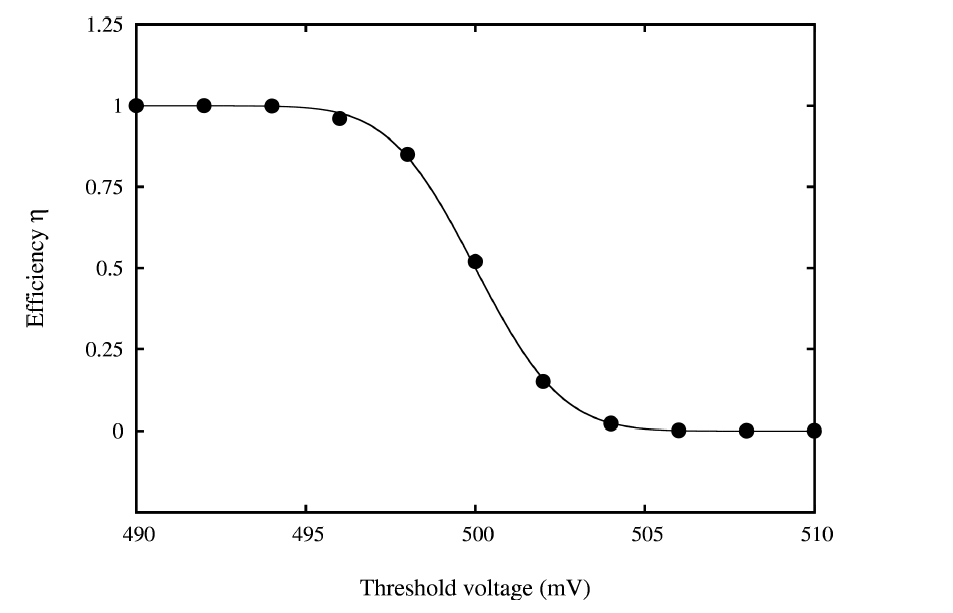
\includegraphics[width=0.65\linewidth]{IMG/ch5/THexample}
	\caption{Example of “S-curve” obtained by scanning the threshold voltage at fixed signal amplitude.}
	\label{fig:thexample}
\end{figure}
%%%%%%%%%%%%%%%%%%%%%%%%%%%%%%%%%%%%%%%%%%%%%%%%%%%%%%%%%%
\paragraph{Measurements}
\noindent
%Before talking about the obtained results it is useful to remember what a threshold scan is and how it is used.
The signal coming from the CSA (Charge Sensitive Amplifier) is a sum of two components, one in DC, that is called the pedestal and can be seen in figure \ref{fig:tscansketch} as a really noisy base, and the signal that is being amplified.
As explained before, the chip sends a logic signal each time the output of the CSA is greater than a selected threshold value.
If the threshold voltage is less than the pedestal the output of the chip will always be \textit{low}, thus the measured rate will be zero.
If the V$_{th}$ is approximately equal to the pedestal the chip will sample noise and the rate will explode.
When the V$_{th}$ is greater than the pedestal the chip is sampling only signal, this can be seen in figure \ref{fig:tscansketch}.
Incrementing even more the threshold voltage will cause a gradual death of the rate, due to the noise. This decrease in the rate can be fitted with an error function, in equation \ref{erf}.
\begin{figure}[H]
	\centering
	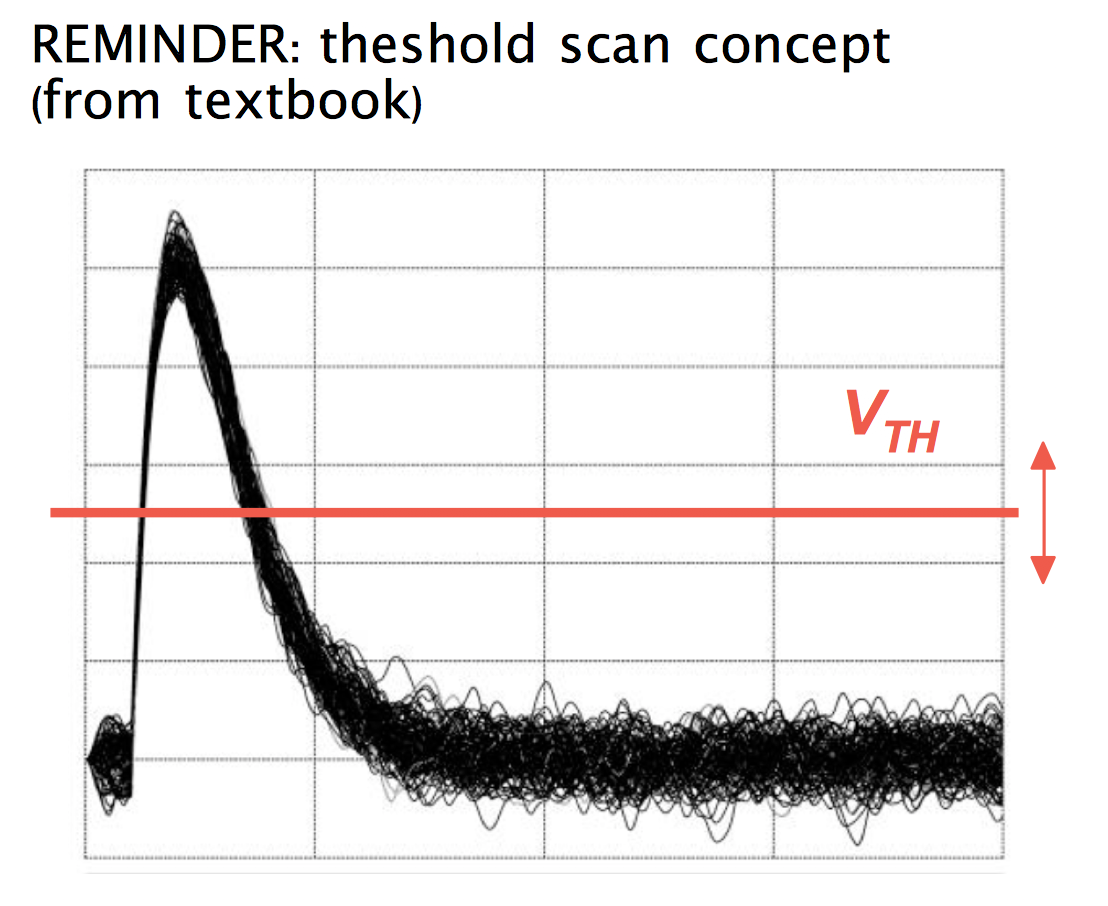
\includegraphics[width=0.7\linewidth]{IMG/ch5/DataDacConfig/tscan_sketch}
	\caption{Threshold scan example from textbook}
	\label{fig:tscansketch}
\end{figure}
\noindent This behaviour can be observed in figure \ref{fig:thscanch0}; in blue there is a threshold scan curve with trimming DAC fixed at 0x00~=~0d00 and variable external DAC, while in green there is the same threshold scan but with trimming DAC setted at 0x3F~=~0d63.
The measurement was performed with the fast pulse generator setted at 600~mV at 10~KHz on the odd channels. The data was extracted from ch1.
It can be observed the conduct described before, at first, for low V$_{th}$, the rate is 0, then in explodes when it reaches the noise; after that it samples the signal, in this case at exactly 10~KHz and lastly it gradually dies. 
By fitting the last part of the threshold scan with and error function it is possible to calculate the pedestal value of the curve.
\noindent The most important thing to observe in figure \ref{fig:thscanch0} is that a change of the trimming DAC value leads to a translation of the threshold scan curve.
This translations is approximately 20~mV.
\begin{figure}[H]
	\centering
	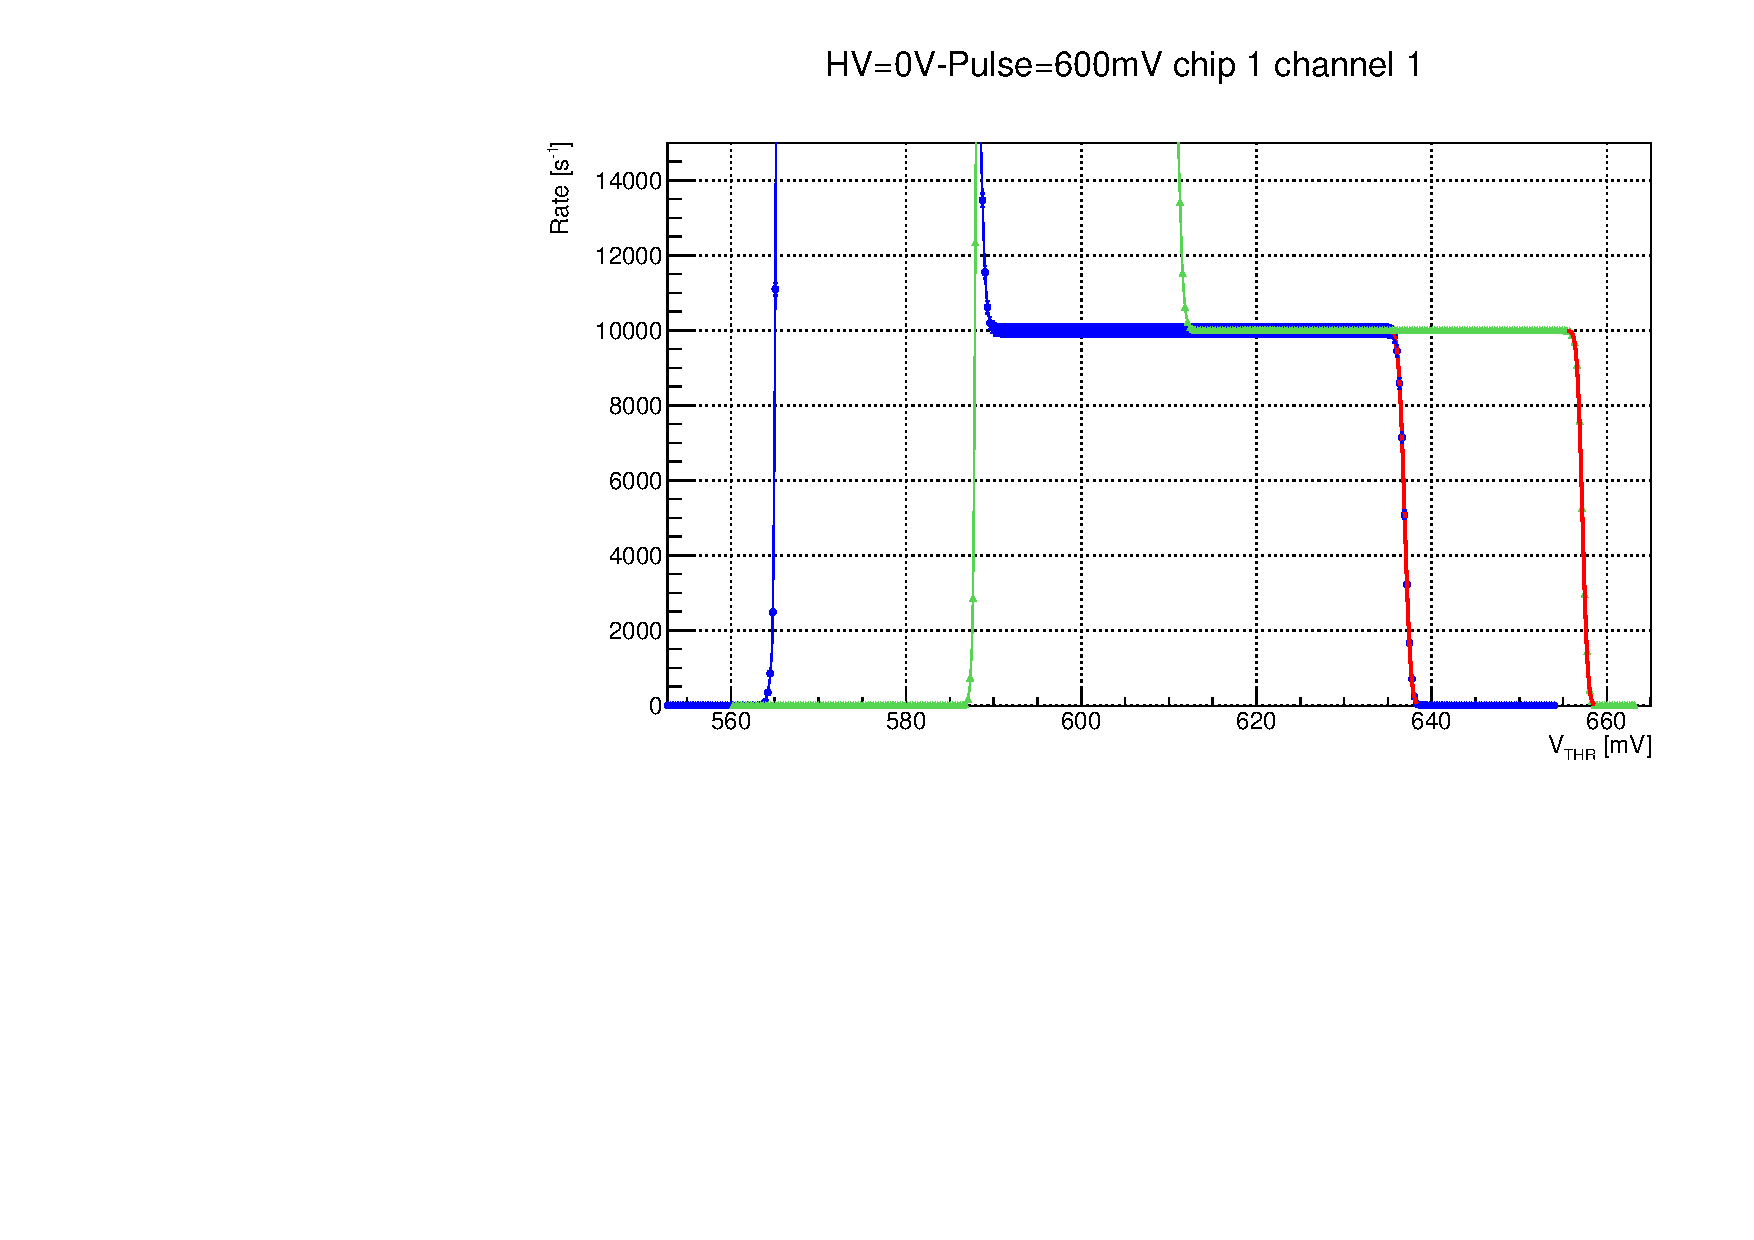
\includegraphics[width=0.7\linewidth]{IMG/ch5/DataDacConfig/ThScan_ch0.pdf}
	\caption{Data analysed by \textit{Emanuele Data}, {\color{blue}blue}= trimming DAC at 0d00,\\{\color{green}green}= trimming DAC at 0d63}
	\label{fig:thscanch0}
\end{figure}

\begin{figure}[H]
	\centering
	\includegraphics[width=0.7\linewidth]{IMG/ch5/DataDacConfig/DAC_V_REF_600mv-Copia.pdf}
	\caption{Data analysed by \textit{Emanuele Data}, {\color{blue}blue}= pedestal values with trimming DAC at 0d00, {\color{green}green}= pedestal values with trimming DAC at 0d63}
	\label{fig:pedestal}
\end{figure}
\noindent After fitting the S-curves with the error function and calculating the pedestal voltages some mode consideration can be taken.
In figure \ref{fig:pedestal} is can be seen a distribution of the pedestal voltages for some channels with trimming DAC configured at 0d00 (blue) and at 0d63 (green).
The average difference between the two values for each channel is approximately 20,9~mV.
In conclusion, the ability to change the trimming DACs values allows to reduce the dis-uniformity between channels and thus to obtain a more accurate measurement of the particles rate.
\newpage
\subsection{Latching counters test}
\textbf{*Warning*} This validation process, as well as the next one, have been performed in a short period of time. This means that the software created for test purposes WON'T be the same used for the future measures. What it will be shown in this sections is a verification of the main features of the new \textit{tera10\_latch\_counter} module. The creation of a LabVIEW data acquisition panel that comprehends every command and control is a complex task that could be the subject of another thesis. \textbf{*Warning*}
\newline
To be noted that this addition to the firmware does not change at all the Input/Output allocation of the board, the only difference is in how the data is being treated; in this case saved into a memory.
In order to test the new \textit{tera10\_latch\_counter} module a new LabVIEW panel (in figure \ref{fig:newlabviewpanel}) was designed by me and the INFN researcher \textit{Simona Giordanengo}.
\begin{figure}[H]
	\centering
	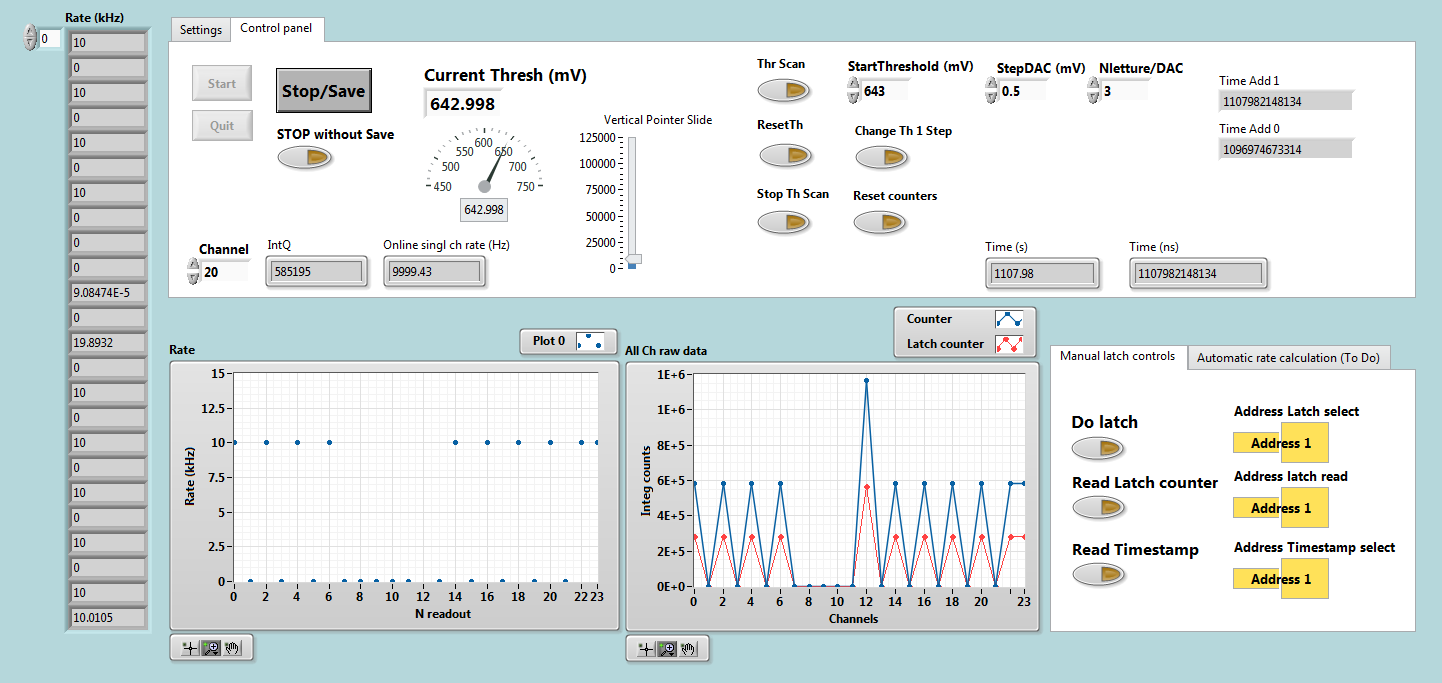
\includegraphics[width=0.99\linewidth]{IMG/ch5/latch_tests/fig1.PNG}
	\caption{New LabVIEW data acquisition panel used for rate measurements}
	\label{fig:newlabviewpanel}
\end{figure}
\noindent This new piece of software allows new types of measurements that could not be done before.
The first two commands tested were: \textit{do\_latch} and \textit{read\_latch\_counter}. The starting point was the already existing \textit{Tera10\_data\_acquisition\_panel}. This LabVIEW piece of software was programmed in such a way to give the user a "real time" reading of every counter [Online singl ch rate (Hz)].
This means that every time the software is running it sends to the FPGA some command that can be: configure a DAC, read a channel, reset, enable or disable selected channels.
When the \textit{DO LATCH} button is pressed a flag is raised, the LabVIEW logic sends the latching command and when it receives the response it goes back to the main state.
In figure \ref{fig:newlabviewpanel} it can be noted that there are two buttons, one for latching and one for reading the counters. For each button there is a boolean controller that allows the selection between address 0 and 1.
By combining the reading and latching addresses four possibilities emerge:
\begin{itemize}
	\item \textbf{LATCH~=~0} and \textbf{READ~=~0 $\rightarrow$} every time the \textit{do\_latch} button is pressed and then the reading command is sent the values displayed are being updated. The user is reading the latest saved latched values.
	\item \textbf{LATCH~=~1} and \textbf{READ~=~0 $\rightarrow$} this time the data is being saved on address 1, however we are still reading from address 0, this means that the data on the screen should stay the same as the case before.
	\item \textbf{LATCH~=~0} and \textbf{READ~=~1 $\rightarrow$} with this combination at the first reading command sent the read data value change, however this happens only the first time. Now the user is writing on address 0 and but reading from address 1. 
	\item \textbf{LATCH~=~1} and \textbf{READ~=~1 $\rightarrow$} this case works as the first one, the user is reading from the same channel on which he is writing thus the data is always updated. 
\end{itemize}
\noindent By doing these four simple tests it turns out that the address system works as intended! The next step is to set the fast pulse generator to a known rate and measure it using the new and improved latch system.
\begin{figure}[H]
	\centering
	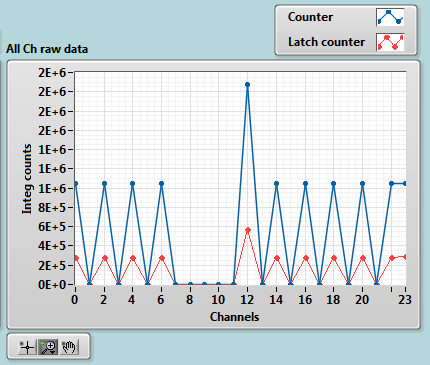
\includegraphics[width=0.5\linewidth]{IMG/ch5/latch_tests/fig2.PNG}
	\caption{Latch counter measurement on graph}
	\label{fig:latchfigure}
\end{figure}
\noindent In figure \ref{fig:latchfigure} it can be seen the behaviour of the latch system. On the X axis there is the channel number and on the Y axis there is the total number of counts; the charge is being sent only to even channels, however it can be seen that not every channel is counting and others, for example \textit{ch23}, are suffering from cross talk problems. Some other channels, like \textit{ch12}, have counts almost doubled. This is known as "counting for after pulse" and happens when the threshold value is not perfectly setted and some noise is being counted.
The key point in this figure is the red line. This is the last read latch value.
When pressing the \textit{Do latch} button the "blue dots" value is saved into the FPGA, when reading the latch this data appears on the graph as "red dots".
These last points are fixed, they do not move if the user does not sends another \textit{Do latch} and \textit{Read Latch counter} command. However, the blue line gradually rises.
This means that doing a latch is like taking a photo of a bunch of moving gauges, it instantly fixes they value without stopping them.  
\subsection{Timestamp generator test}
\noindent \textbf{*Warning*} This section, as the previous one, is not a demonstration of the complete capabilities of the new timestamp generator, instead it is a proof of the correct operation of the device. Future work on the project will expand the LabVIEW data acquisition system and use at his full extend this new module. \textbf{*Warning*}
\newline
As explained in chapter 4, the timestamp generator appears like a 64~bit that can be read in four 16~bit sections.
With the help of INFN researcher \textit{Simona Giordanengo} I updated the data acquisition panel in order to implement the \textit{read\_timestamp} command.
The final LabVIEW piece of software that can be seen in figure \ref{fig:newlabviewpanel} has also a button to read the timestamp and a boolean controller to select the address.
The read value is shown as an integer in indicators \textit{Time add 1} and \textit{Time add 2}. The last read timestamp is also converted in nanoseconds~(\textit{ns}) and in seconds~(\textit{s}).
To be noted that the timestamp can NOT be restarted, it starts from zero when the boards turns on and always counts, thus the \textit{Time~(s)} could also be a "\textit{Wake time}" indicator.
These values can be seen in figure \ref{fig:timestampfigure}
\begin{figure}[H]
	\centering
	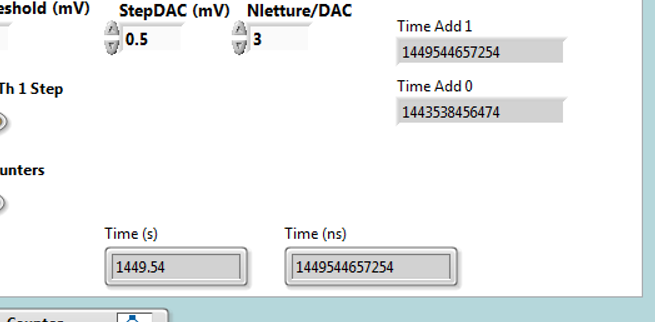
\includegraphics[width=0.5\linewidth]{IMG/ch5/latch_tests/fig15.PNG}
	\caption{Details of the Timestamp indicators values. For example in this case the timestamp measurement was done $\approx$~24~min after the board was turned on}
	\label{fig:timestampfigure}
\end{figure}
\noindent A proper performance test of this new feature is presented in the next subsection. However, a simple measurement was performed in order to check if the timestamp counter runs at a "reasonable speed".
This was done simply by saving the timestamp data and starting a chronometer at the same time. After a defined time, in this case half an hour (1800~s), the new timestamp reading should be incremented of the same 1800~s.
This is exactly what happened, thus the timestamp module is working as intended.  
\begin{figure}[H]
	\centering
	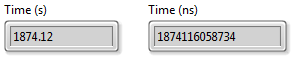
\includegraphics[width=0.35\linewidth]{IMG/ch5/latch_tests/fig20.PNG}
	\caption{Timestamp measured after 30 min = 1800 s\\initial time $\approx$ 74.1 s}
	\label{fig:timestamptest}
\end{figure}

\subsection{Rate measurements}\label{RateMeasurements}
\noindent In this section it will be shown the results of the rate measurements. in order to do so two instants (states) were saved with the latch system on the two different addresses. Using formula \ref{eq:rate} the rate was calculated for each channel and the plotted.
\begin{equation}\label{eq:rate}
	Rate\:=\: \frac{\Delta N_i}{\Delta T}
\end{equation}
\noindent With $N_i$ the number of counts at the $i^{th}$ channel and $\Delta T$ the difference between the two saved timestamps.
In figures \ref{fig:latchrate10} \ref{fig:latchrate50} \ref{fig:latchrate75} \ref{fig:latchrate110} it can be seen a graph for each impulsed frequency. On the X axis there is the channel number and on the Y axis there is the calculated rate in kHz. It can be observed that the even channels that are counting have a measured rate that is perfectly compatible with the theoretical one.
The biggest discrepancy appears in figure \ref{fig:50khz} where against a sent frequency of 50~kHz, one of 49.9998~kHz is measured. The difference is 0.2~Hz, which is less than the 1\% clinical tolerance. However much more measurements and test are needed in order to calculate the precision of those numbers.
It is noteworthy the behaviour of \textit{ch23}. This is an odd channel, it does not receive any charge, however it is counting. This is due to cross-talk effects.
From the figures shown earlier it emerges that this behaviour becomes less and less pronounced at higher rate.
If in the first case (figures \ref{fig:latchrate10} and \ref{fig:10khz}) the measured rate is almost 100\% of the sent one, in the next tests this value drops to:
63.1\% for the 50~kHz case (figures \ref{fig:latchrate50} and \ref{fig:50khz}),
55,8\% for the 75~kHz case (figures \ref{fig:latchrate75} and \ref{fig:75khz}) and
42.5\% for the 110~kHz case (figures \ref{fig:latchrate110} and \ref{fig:110khz}).
\newline
\noindent \textbf{*Warning*} These measurements where made by pressing in the proper order the three buttons of the \textit{Manual latch controls} tab of figure \ref{fig:newlabviewpanel}.
This process is not yet automated, thus there is no consistency between the time difference ($\Delta T$) of the two latched states.
In ideal conditions, like the ones of the lab, this is not a problem because the fast pulse generator sends always a constant rate.
However the next important step is to create an automated rate calculation logic in LabVIEW that can automatically send the commands to the FPGA with a setted, precise and configurable delay. \textbf{*Warning*}
%%% [!htpb]
\begin{figure}[H]
	\centering
	\begin{minipage}{0.49\textwidth}
		\centering
		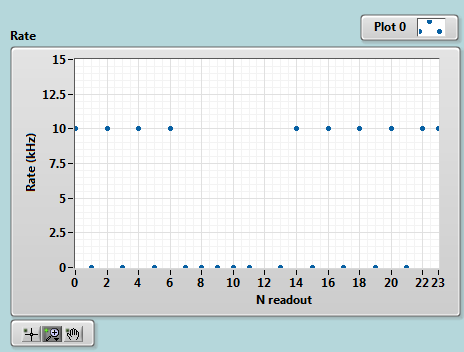
\includegraphics[width=.95\linewidth]{IMG/ch5/latch_tests/fig3.PNG}
		\caption{Latch Rate calculation at 10~kHz impulse rate}
		\label{fig:latchrate10}
	\end{minipage}%
	\begin{minipage}{0.49\textwidth}
		\centering
		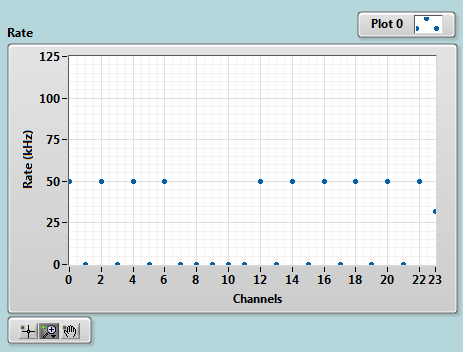
\includegraphics[width=.95\linewidth]{IMG/ch5/latch_tests/fig5.PNG}
		\caption{Latch Rate calculation at 50~kHz impulse rate}
		\label{fig:latchrate50}
	\end{minipage}
\end{figure}
\begin{figure}[H]
	\centering
	\begin{minipage}{0.49\textwidth}
		\centering
		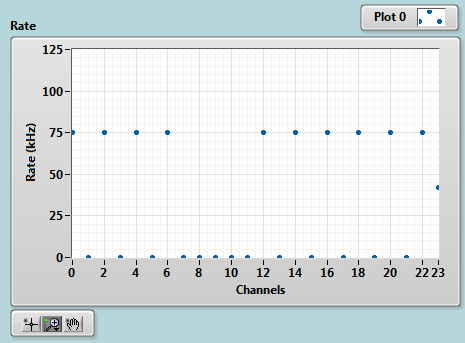
\includegraphics[width=.95\linewidth]{IMG/ch5/latch_tests/fig9.PNG}
		\caption{Latch Rate calculation at 75~kHz impulse rate}
		\label{fig:latchrate75}
	\end{minipage}%
	\begin{minipage}{0.49\textwidth}
		\centering
		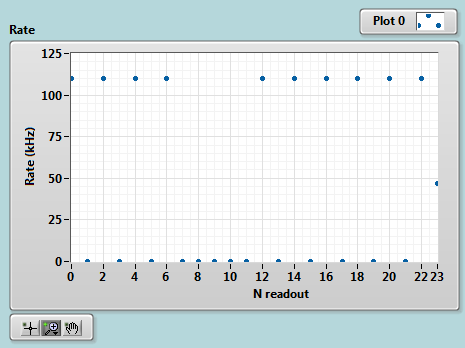
\includegraphics[width=.95\linewidth]{IMG/ch5/latch_tests/fig12.PNG}
		\caption{Latch Rate calculation at 110~kHz impulse rate}
		\label{fig:latchrate110}
	\end{minipage}
\end{figure}







\begin{figure}[H]
	\centering
	\begin{minipage}{0.24\textwidth}
		\centering
		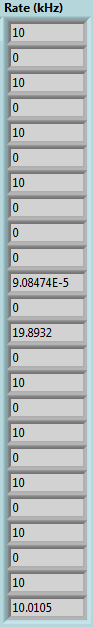
\includegraphics[width=.75\linewidth]{IMG/ch5/latch_tests/fig16}
		\caption{Pulsed rate=\\10~kHz}
		\label{fig:10khz}
	\end{minipage}
	\begin{minipage}{0.24\textwidth}
		\centering
		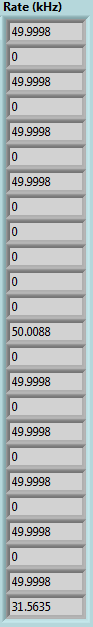
\includegraphics[width=.75\linewidth]{IMG/ch5/latch_tests/fig17}
		\caption{Pulsed rate=\\50~kHz}
		\label{fig:50khz}
	\end{minipage}
	\begin{minipage}{0.24\textwidth}
		\centering
		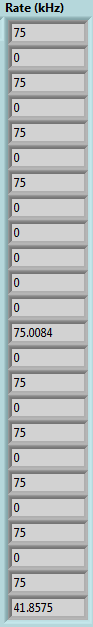
\includegraphics[width=.75\linewidth]{IMG/ch5/latch_tests/fig18}
		\caption{Pulsed rate=\\75~kHz}
		\label{fig:75khz}
	\end{minipage}
	\begin{minipage}{0.24\textwidth}
		\centering
		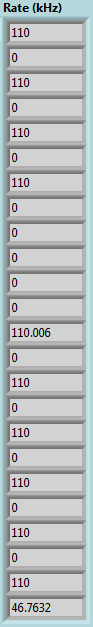
\includegraphics[width=.75\linewidth]{IMG/ch5/latch_tests/fig19}
		\caption{Pulsed rate=\\110~kHz}
		\label{fig:110khz}
	\end{minipage}
\end{figure}







